\chapter{FUNDAMENTOS TEÓRICOS}
\cpnote{Quizá evitaría hacer una sección que se llame introducción. simplemente
haría de la seccion ``ensambles de estados cuánticos'', la sección 1.1. Lo mismo para los 
siguientes capítulos. Si estas de acuerdo, no mas sería comentar la linea que marca
la introducción.}
\section{Introducción} % {{{
% \esqueleto{Escribiré que la matriz de densidad
% y la teoría de canales cuánticos es el marco teórico para el problema 
% de las operaciones PCE. Luego un enunciado que resuma de manera
% introductoria la idea de cada uno de los conceptos. \newline\newline
% Por último enunciar la estructura del capítulo.}

Para estudiar las operaciones de Pauli que borran componentes (PCE)
se necesitan herramientas matemáticas para describir a los estados 
cuánticos y su evolución dinámica\cpnote{Me parece una forma mala de abrir la tesis. 
La gente no sabe que es eso. Supongo que lo introduciras más adelante. Yo sugeririra
quitar ese término (PCE) y rediseñar estas primeras dos frases. Quizá 
mejor motivalo desde los sistemas abiertos o desde mediciones que es el objeto 
fundamental de nuestro estudio. Marcame todo el párrafo para revisar cuando lo iteres.}. Nuestro
interés en el problema de 
las operaciones PCE se enfoca para los sistemas cuánticos abiertos, 
sistemas que interaccionan con otro sistema externo. Por ello recurrimos
a la teoría de los canales cuánticos como marco teórico para estudiar 
la dinámica. En este marco teórico los estados cuánticos se representan
por medio de su matriz de densidad, un formalismo distinto pero equivalente
al del vector de estado. Estas dos herramientas cuentan con las características 
necesarias para analizar el problema de las operaciones que borran
componentes de Pauli de la matriz de densidad de un sistema de qubits.

La estructura de este capítulo es la siguiente. En la sección \ref{sec:ensambles}
vamos a presentar la motivación física que conduce a introducir
la matriz de densidad. La caracterización, una reformulación de los 
postulados de la mecánica cuántica y una de las aplicaciones más 
importantes de la matriz de densidad lo presentamos en la sección
\ref{sec:density-matrices-properties}. Por último, 
en las secciones \ref{sec:qtm-channels}
y \ref{sec:qtm-channels-representation} presentamos la teoría de los
canales cuánticos y dos formas en las que se puede representar
a un canal cuántico, respectivamente.
% }}}
\section{Ensambles de estados cuánticos} \label{sec:ensambles} % {{{
\esqueleto{Un copy-paste de la sección 1.1 del informe final de 
prácticas. Voy a retocar alguna parte si fuera necesario, como ser
más formal o agregar alguna prueba.}

Para introducir la definición del operador de densidad presentamos la 
motivación que exponen Sakurai y Napolitano \cite{sakurai_napolitano_2017}.
Consideremos un sistema cuántico que se encuentra en alguno de los estados 
$\Pk{i}$ con probabilidad $p_i$. El conjunto de todos los posibles estados
conforman un ensamble de estados del sistema. Supongamos que realizamos 
la medición de algún observable $\Lambda$ sobre el ensamble. El 
valor esperado al medir $\Lambda$ sobre este sistema se encuentra
\begin{align}\label{eq:expVal-expanded-Lambda}
	\expval{\Lambda} &= \sum_i p_i \matrixel{\psii}{\Lambda}{\psii}\nonumber\\
	&= \sum_{i,j,k} p_i 
	\bra{\psii}\dyad{\phi_j}{\phi_j}\Lambda\dyad{\varphi_k}{\varphi_k}\Pk{i},
\end{align}
con $\ket{\phi_j}$ y $\ket{\varphi_k}$ dos bases ortonormales distintas del
espacio de Hilbert del sistema. Ahora, al reordenar 
\eqref{eq:expVal-expanded-Lambda} se obtiene una expresión 
que motiva claramente la definición de la matriz de densidad $\rho$,
\begin{align}\label{eq:expVa-Lambda-wRho}
	\expval{\Lambda}&= \sum _{j,k}\bra{\varphi_k}\qty(\sum_ip_i \dyad{\psii}{\psii} 
	)\ket{\phi_j}	\matrixel{\phi_j}{\Lambda}{\varphi_k}.
\end{align}
La matriz que se encuentra dentro del paréntesis se define como 
la matriz de densidad 
$\rho$~\cite{nielsen_chuang_2011, sakurai_napolitano_2017}
\begin{equation}
	\rho \equiv \sum _i p_i\dyad{\psi_i}{\psi_i}.
	\label{eq:rho_def}
\end{equation}
Notemos que 
\begin{align}
	\matrixel{\varphi_k}{\rho}{\phi_j} = 
	\sum_ip_i \braket{\varphi_k}{\psii}\braket{\psii}{\phi_j},
\end{align}
por lo tanto, sustituyendo en la ecuación \eqref{eq:expVa-Lambda-wRho},
se tiene
\begin{align}\label{eq:Tr(rhoLambda)}
	\expval{\Lambda}=\sum _k \matrixel{\varphi_k}{\rho \Lambda}{\varphi_k} 
	= \Tr \qty(\rho\Lambda).
\end{align} 
Este resultado muestra que la matriz de densidad $\rho$ 
contiene toda la información física disponible de un sistema al 
realizar una medición.

Desde luego la matriz de densidad es una herramienta con la que
se puede formular matemáticamente la mecánica cuántica como 
con el vector de estado. Por ejemplo, veamos a continuación cómo 
describir la evolución de un sistema cuántico cerrado.
Consideremos un sistema cuyo Hamiltoniano es $H$, y es
independiente del tiempo. Bajo estas condiciones la evolución
del sistema está descrita por 
$\ket{\psi (t)}=e^{-iHt/\hbar}\ket{\psi(0)}$~\cite{sakurai2010modern}. 
Sin embargo, consideremos que el sistema se encuentra inicialmente
en un ensamble de estados $\{p_i, \ket{\psii(0)}\}$, por lo cual
el estado final del sistema será 
$\{p_i, \ket{\psii(t)}\}$.
Por consiguiente, el operador de densidad final $\rho(t)$  es 
\begin{align} \label{eq:Rho-evolution-H}
	\rho(t) &= \sum_j p_j\dyad{\psi_j(t)}{\psi_j(t)}\nonumber\\
	&= \sum_j p_j e^{-iHt} \dyad{\psi_j(0)}{\psi_j(0)}\qty(e^{-iHt})^{\dagger}
	\nonumber\\
	&= e^{-iHt}\rho(0)e^{iHt},
\end{align}
donde $\rho(0)$ es la matriz de densidad que describe al ensamble 
de estados inicial $\{p_i, \ket{\psii(0)}\}$.	 Aunque hemos desarrollado 
un ejemplo para la evolución de un sistema cuyo Hamiltoniano es 
independiente del tiempo, es sencillo de ver que en general la dinámica  
de un sistema cerrado se describe como 
\begin{align}\label{eq:rho-ClosedEvolution}
\rho(0) \longrightarrow U\rho(0)U^{\dagger}.
\end{align}
Con esto, se ha asegurado que la dinámica de un sistema cuántico puede 
describirse utilizando su matriz de densidad.

Las ecuaciones \eqref{eq:Tr(rhoLambda)} y \eqref{eq:rho-ClosedEvolution}
muestran que la matriz de densidad puede utilizarse para la descripción 
de la medición y la evolución de los estados cuánticos. 
En la siguiente sección veremos la formulación de los postulados 
de la mecánica cuántica utilizando la matriz de densidad.

% }}}
\section{Propiedades de la matriz de densidad} % {{{
\label{sec:density-matrices-properties}
\esqueleto{Revisando esta sección en el informe de prácticas 
veo que me gustaría ir aquí más al grano y mandar al lector 
a las pruebas en el Chuang (para no copiar otra vez las pruebas
aquí). Puntualizaré: (1) caracterización de la matriz de densidad, (2)
postulados de la mecánica cuántica usando la matriz de densidad y
(3) matriz de densidad reducida. Para la matriz de densiddad reducida
voy a omitir el ejemplo que coloqué en el informe de prácticas.}



Según Nielsen y Chuang \cite{nielsen_chuang_2011} las matrices
de densidad están caracterizadas por el siguiente teorema:
\begin{thm}\label{teo:density-operator}
Un operador $\rho$  que actúa sobre el espacio de Hilbert de un sistema 
es el operador de densidad asociado a algún ensamble 
$\{p_i, \ket{\psi _i} \}$ si y sólo si satisface las condiciones:
\begin{enumerate}
\item $\Tr \rho = 1$.
\item $\rho \geq 0$.
\end{enumerate}	
\end{thm} 
\begin{proof} Consultar~\cite[p.~101]{nielsen_chuang_2011} \end{proof}

La condición de traza unitaria de la matriz de densidad cumple la misma
función que la condición de normalización del vector de estado. La
suma de las probabilidades de todas las posibles mediciones 
de un observable deben sumar uno. La condición de positividad 
implica que los eigenvalores $\lambda_i$ y eigenvectores
$\ket{i}$ dan lugar a $\{\lambda_i, \ket{i}\}$, uno de todos los 
posibles ensambles que están asociados a la matriz de densidad $\rho$.

Ahora que hemos establecido de manera precisa a la matriz de densidad
nos ocupamos de la formulación de los postulados de la mecánica cuántica 
utilizando la matriz de densidad \cite[p.~102]{nielsen_chuang_2011}.
\begin{itemize}
	\item[] \textbf{Postulado 1.} \textit{Estado del sistema.} 
	Un sistema físico tiene asociado un espacio vectorial complejo
	con producto interno que se conoce como el espacio de Hilbert $\hi$ del
	sistema. Los estados del sistema están descritos por el conjunto 
	de matrices de densidad en el espacio de Hilbert-Schmidt $\mathcal{HS}$	
	que actúan sobre el espacio de Hilbert $\hi$ del sistema. 
	\item[] \textbf{Postulado 2.} \textit{Evolución unitaria.}
	La evolución de un sistema cuántico cerrado en un intervalo 
	de tiempo $[t_1,t_2]$ está descrita 	por una transformación unitaria
	de la siguiente manera 
	\begin{equation} \label{eq:postulate-ClosedEvolution}
	\rho(t_1)\longrightarrow U\rho(t_1) U^{\dagger}=\rho(t_2).
	\end{equation}
	\item[] \textbf{Postulado 3.} \textit{Medición.}
	Las mediciones están descritas por un conjunto de 
	operadores $\{M_m\}$. Estos son operadores que actúan sobre el espacio 
	de Hilbert $\hi$ del sistema. El índice $m$ refiere a los posibles
	resultados de la medición. Si el estado del sistema es $\rho$ 
	inmediatamente antes de la medición, entonces la probabilidad
	de medir $m$ es
	\begin{equation} \label{eq:post_MeasureProb}
	p(m)=\Tr \qty(M_m^{\dagger}M_m\rho),
	\end{equation}						
	y el estado del sistema después de la medición será
	\begin{equation} \label{eq:post_MeasureTrasnfState}
	\rho'=\frac{M_m\rho M_m^{\dagger}}{\tr \qty(M_m^{\dagger}M_m\rho)}.
	\end{equation}	
	Los operadores $M_m$ deben satisfacer la ecuación de completitud
	\begin{equation} \label{eq:post_MeasureMCompleteness}
	\sum _m M_m^{\dagger}M_m=\mathbb{1}.
	\end{equation}
%	Este postulado confirma lo que en la sección anterior aseguramos
%	de que la formulación de cualquier medición proyectiva utilizando el 
%	operador de densidad es posible. Debemos notar que las mediciones
%	proyectivas son un caso especial de las mediciones enunciadas en
%	este postulado.
%	Una medición proyectiva está descrita por un observable
%	$\Omega$, que es un operador Hermítico que actúa sobre $\hi$. 
%	$\Omega$ tiene una descomposición espectral \cite{nielsen_chuang_2011}
%	\begin{align}
%		\Omega = \sum _i \lambda_iP_i,
%	\end{align}
%	donde $P_i$ es el proyector al autoespacio de $\Omega$ 
%	con autovalor $\lambda_i$.
%	De acuerdo con este postulado si el sistema se encuentra en el estado
%	$\rho$, la probabilidad de medir $\lambda_i$ es
%	\begin{align}
%		p(i) = \Tr \qty(P_i^{\dagger}P_i\rho) = \Tr \qty(P_i\rho).
%	\end{align}
%	Además, dado que se midió $\lambda_i$ el estado del sistema inmediatamente 
%	luego de realizar la medición es 
%	\begin{align}
%		\rho'&=\frac{P_i\rho P_i}{\Tr \qty(P_i \rho)}.
%	\end{align}
	\item[] \textbf{Postulado 4.} \textit{Sistemas de partículas.}
	El espacio de Hilbert de un sistema 	de varias partículas se compone del
	producto tensorial de los espacios de Hilbert 	individuales.
	Es decir, si el sistema total se compone de $N$ partículas, 
	entonces el sistema total es
	\begin{align}
		\hi_{\txt{total}} = \hi_1\ten \hi_2 \ten \ldots \ten \hi_N.
	\end{align}
	Los estados del sistema total están descritos por las matrices de 
	densidad que actúan sobre $\hi _{\text{total}}$.
\end{itemize}

Por último en esta sección discutiremos sobre la matriz de densidad
reducida, una herramienta especialmente útil para los sistemas 
de varias partículas. La matriz de densidad es una herramienta 
que proporciona toda la información física disponible al hacer 
una medición sobre cualquier parte del sistema total. 

Supongamos dos subsistemas $A$ y $B$ cuyo estado total es 
$\rho^{AB}$ (en general, $\rho^{AB}\neq \rho^A\ot \rho^B$). 
Consideremos una base ortonormal $\ket{\psi_i}$ de $A$ y una 
base ortonormal $\ket{\phi_j}$ de $B$. Una base ortonormal 
del sistema total está dado por el producto tensorial entre los elementos
de la base de A y de B. En esta base, un elemento de matriz
de $\rho^{AB}$ está dado por
\begin{align}
	\bra{\psi_i}\ten\bra{\phi_j}\rho^{AB}\ket{\psi_k}\ten\ket{\phi_l}.
\end{align}
Supongamos que $\Omega_A$ es un observable únicamente de $A$
que actúa sobre el espacio de Hilbert total. El valor esperado de 
$\Omega_A$, utilizando \eqref{eq:Tr(rhoLambda)}, es
\begin{align}
	\Tr \qty(\rho^{AB}\qty(\Omega_A\ot \mathbb{1})) &= \sum _{i,j} 
	\bra{\psi_i}\bra{\phi_j}\rho^{AB}\qty(\Omega_A\ot \mathbb{1})
	\ket{\psi_i}\ket{\phi_j} 
	\nonumber\\
	&= \sum _{i,j} 
	\bra{\psi_i} \bra{\phi_j}\rho^{AB}
	\qty(\sum _{k,l} \ket{\psi_k} \dyad{\phi_l}
	\bra{\psi_k} \bra{\phi_l} )
	\qty(\Omega_A\ot \mathbb{1})\ket{\psi_i} \ket{\phi_j}\nonumber\\
	&= \sum _{i,j,k,l} 
	\bra{\psi_i} \bra{\phi_j}\rho^{AB}\ket{\psi_k} \ket{\phi_l}
	\matrixel{\psi_k}{\Omega_A}{\psi_i}\delta _{lj}\nonumber\\
	&= \sum_{i,k}\qty(\sum _j 
	\bra{\psi_i} \bra{\phi_j}\rho^{AB}\ket{\psi_k} \ket{\phi_j})
	\matrixel{\psi_k}{\Omega_A}{\psi_i},
	\label{eq:almost-reducedRho}
\end{align}
donde hemos utilizado $\ket{\psi}\ot\ket{\phi}=\ket{\psi}\ket{\phi}$.
De lo que está entre paréntesis definimos a la matriz de densidad
reducida $\rho^A$ como~\cite{chandra2013quantum}
\begin{align}
	\sum _j \bra{\psi_i}\bra{\phi_j}\rho^{AB}\ket{\psi_k}\ket{\phi_j}
	= \matrixel{\psi_i}{\rho^A}{\psi_k}.
	\label{eq:reducedRho-def1}
\end{align}
Con $\rho^A$ definido retomemos  \eqref{eq:almost-reducedRho}
\begin{align}
	\Tr \qty(\rho^{AB}\qty(\Omega_A\ot \mathbb{1}))&= \sum _{i,k}\nonumber
	\matrixel{\psi_i}{\rho^A}{\psi_k} \matrixel{\psi_k}{\Omega_A}{\psi_i}
	\nonumber\\
	&= \sum_i \matrixel{\psi_i}{\rho^A\Omega_A}{\psi_i}\nonumber\\
	&= \Tr \qty(\rho^A\Omega_A). \label{eq:reduced-works}
\end{align}
Este resultado es similar al que se obtuvo en la ecuación
\eqref{eq:Tr(rhoLambda)}, por lo cuál nos conduce a una
conclusión similar. La matriz de densidad reducida $\rho^A$ 
contiene la información que se puede extraer al 
hacer una medición exclusivamente del subsistema $A$.

La operación que define a la matriz de densidad reducida en 
la ecuación \eqref{eq:reducedRho-def1} se conoce como la traza parcial
\begin{align} 
	\sum _j \bra{\psi_i}\bra{\phi_j}\rho^{AB}\ket{\psi_k}\ket{\phi_j}
	&=\matrixel{\psi_i}{\Tr_B\qty(\rho^{AB})}{\psi_k}
	= \matrixel{\psi_i}{\rho^A}{\psi_k}.
	\label{eq:partialTrace-def}
\end{align}
%\janote{aquí voy} \janote{hablar de que la traza parcial es trazar 
%sobre los grados de libertad que no intersan}
De manera precisa la traza parcial se define como \cite{nielsen_chuang_2011}
\begin{align}
	\Tr_B (\dyad{\alpha_i}{\alpha_j}\otimes \dyad{\beta_k}{\beta_l})
	\equiv
	\dyad{\alpha_i}{\alpha_j}\braket{\beta_k}{\beta_l},
	\label{eq:part_trace-def}
\end{align}
donde $\ket{\alpha_i}$ son vectores ortonormales del subespacio $\hi_A$
y $\ket{\beta_j}$ del resto del espacio de Hilbert total. En sistemas 
multipartitos la traza parcial se puede entender como la traza sobre 
todos los grados de libertad del sistema, excepto los del subsistema de interés. 

%Es sencillo probar
%que, ya que la traza es una operación lineal, la traza parcial también 
%lo es. 
%Además, debe notarse en la deducción que se presentó para motivar 
%al operador de densidad recudido, 
%que la ecuación \eqref{eq:reducedRho-def1} evidencia 
%el uso de la traza parcial, definida en \eqref{eq:part_trace-def}, 
%como la única operación que da lugar al operador de densidad reducido. 

%Antes de concluir revisaremos un ejemplo del cálculo del 
%operador de densidad reducido que evidencia una de las
%\textit{extrañas} consecuencias del
%entrelazamiento cuántico.
%Consideremos un sistema de 2 qubits que se encuentra en el estado de Bell
%$\qty(\ket{00}-\ket{11})/\sqrt{2}$, un estado entrelazado. El operador
%de densidad para el sistema compuesto es
%\begin{align}
%	\rho &= \qty(\frac{\ket{00}-\ket{11}}{\sqrt{2}})
%	\qty(\frac{\bra{00}-\bra{11}}{\sqrt{2}}) \\
%			 &= \frac{\dyad{00}{00}-\dyad{11}{00}-\dyad{00}{11}
%                 +\dyad{11}{11}}{2}.
%\end{align}
%Calculamos ahora el operador de densidad reducido para el qubit 1.  
%Haciendo la traza parcial sobre el qubit 2 se tiene
%\begin{align}
%	\rho^A &= \Tr _B(\rho) \\
%			 	 &= \frac{\Tr _B(\dyad{00}{00})-\Tr _B(\dyad{11}{00})
%			 	 -\Tr _B(\dyad{00}{11})+\Tr _B(\dyad{11}{11})}{2} \\
%			 	 &= \frac{\dyad{0}{0} + \dyad{1}{1}}{2} \\
%			 	 &= \frac{\mathbb{1}}{2}.
%\end{align}
%Notemos que el qubit 1 se encuentra en un estado mixto
%$\qty(\Tr \qty(\mathbb{1}/2)^2<1)$. De hecho, si hiciéramos la 
%traza parcial sobre el qubit 1 llegaríamos al mismo estado del qubit 2.
%Es decir, aunque contamos con la información completa del estado 
%de los dos qubits como sistema compuesto, tenemos incompleta la 
%información del estado individual de cualquiera de los dos qubits
%en el sistema. Esta es una de las consecuencias del entrelazamiento
%cuántico.

La matriz de densidad reducida completa todo lo que necesitamos 
saber de la matriz de densidad reducida para continuar con la descripción
de la evolución de los estados cuánticos en la siguiente sección. 
La matriz de densidad, caracterizada como una matriz positiva de traza unitaria, 
es una herramienta para representar a los estados cuánticos y, junto 
con la matriz de densidad reducida, proporcionan 
la información accesible al observador de un sistema, 
completo o cualquier parte de él. 

% }}}
\section{Canales cuánticos}\label{sec:qtm-channels} % {{{
\esqueleto{Copy-paste del informe final, sección mapeos 
completamente positivos.}

Los sistemas cuánticos reales sufren de interacción con su entorno.
Por esa razón, se hace necesario un marco teórico para describir 
la evolución de los sistemas cuánticos abiertos. Una de las propuestas
para ello es la teoría de los canales cuánticos que describe la dinámica de 
los sistemas abiertos de forma discreta. 

La teoría de los canales cuánticos ocupa a la matriz de densidad para 
representar a los estados cuánticos. Esta teoría establece que un 
sistema que se encuentra en un estado $\rho$ se transforma a un 
estado final $\rho'$ descrito por un canal cuántico
$\E$, según la ecuación~\cite{nielsen_chuang_2011}
\begin{align} \label{eq:E(rho)}
\rho' = \E (\rho),
\end{align} 
Evidentemente, $\E$ debe ser una operación lineal 
que preserva las características de la matriz de densidad: (1) traza
unitaria y (2) positividad. Sin embargo, hace falta una condición 
más sobre $\E$ para que describa una evolución física. El sistema
principal ($P$) podría encontrarse en un estado entrelazado 
$\rho^{\text{total}}$ $(\rho^{\text{total}}\neq \rho^P\ot\rho^S)$ 
con un sistema secundario ($S$). La condición adicional sobre $\E$ 
debe asegurar que, para cualquier sistema secundario, el operador $\E\ot\1$ 
también preserva la positividad de la matriz de densidad, especialmente 
la de los estados entrelazados (como $\rho^{\text{total}}$). Esta 
condición se conoce como completa positividad (CP).

Para entender mejor la condición de CP vamos a revisar un 
ejemplo. Vamos a considerar la operación lineal $\E_z$ de 1 qubit (partícula
de espín 1/2) que mapea la bola de Bloch a un disco perpendicular 
al eje $z$ (\Fref{fig:qtm-op-motivation}). 
Seguidamente, veremos que $\E_z \ot\1$ no preserva la
positividad del estado máximamente entrelazado (estado de Bell)
de 2 qubits.

Para escribir a la matriz de densidad utilizaremos 
la base de produtos tensoriales de las matrices de Pauli
$\{ \sigma_0, \sigma_1, \sigma_2, \sigma_3\}$,
con $\sigma_0=\1$ y los subíndices $1,2,3$ para etiquetar a $x$, $y$ y $z$.
Respectivamente, las matrices de densidad para 1 y 2 qubits se 
escriben como~\cite{nielsen_chuang_2011}
\begin{align}
\rho^1&=\frac{1}{2}\sum_{i=0}^{3} r_i\sigma_i,
& 
\rho^2&=\frac{1}{4}\sum _{i,j=0, }^{3}r_{ij}\sigma_i\otimes\sigma_j,
\label{eq:densityMatrices_1and2Qubits}
\end{align}
donde $r_0=r_{00}=1$ $(\Tr\rho=1)$.
Las componentes $r_i$ y $r_{ij}$ definen un vector de 4 entradas
y una matriz de $4\times4$.
Para 1 qubit, las componentes $\qty(r_1, r_2, r_3)$ definen 
un punto en la bola de Bloch.
En el panel izquierdo de la \Fref{fig:qtm-op-motivation} 
se muestra a la bola de Bloch y algunos estados de 1 qubit. 
Los estados puros se corresponden con puntos en la superficie
y los estados mixtos con puntos en el interior.


La transformación de la matriz de densidad de 1 qubit bajo la acción 
de  $\E_z$ es sencilla en términos de las componentes $r_i$
de $\rho^1$ en \eqref{eq:densityMatrices_1and2Qubits}.
La operación $\E_z$ transforma a las componentes de $\rho^1$ como
$\qty(1,r_1,r_2,r_3)\mapsto\qty(1,r_1,r_2,0)$. De la \Fref{fig:qtm-op-motivation}
podemos notar que todos los puntos del disco son estados de 1 qubit, por 
lo cual es bastante intuitivo entender que $\E_z$ preserva la positividad y 
la traza unitaria de todos los estados de 1 qubit. 
Sin embargo, veremos a continuación que el estado 
máximamente entrelazado de 2 qubits se transforma en una 
matriz no positiva.

\begin{figure}% {{{
\centering
\begin{minipage}{.4\textwidth}
\centering
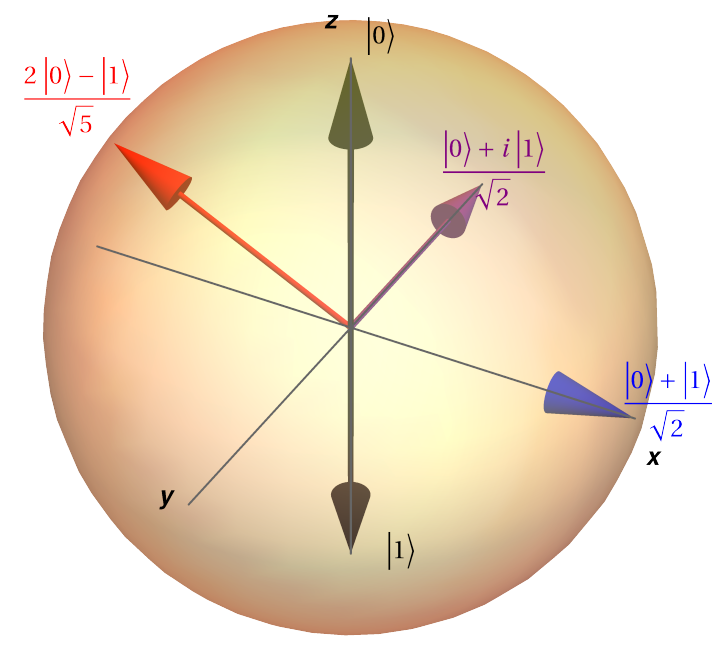
\includegraphics[width=5cm]{bloch.png}
\end{minipage}
$\stackrel{\E_{z}\otimes\1 \vspace{1cm}}{\longmapsto}$
\begin{minipage}{0.4\textwidth}
\centering
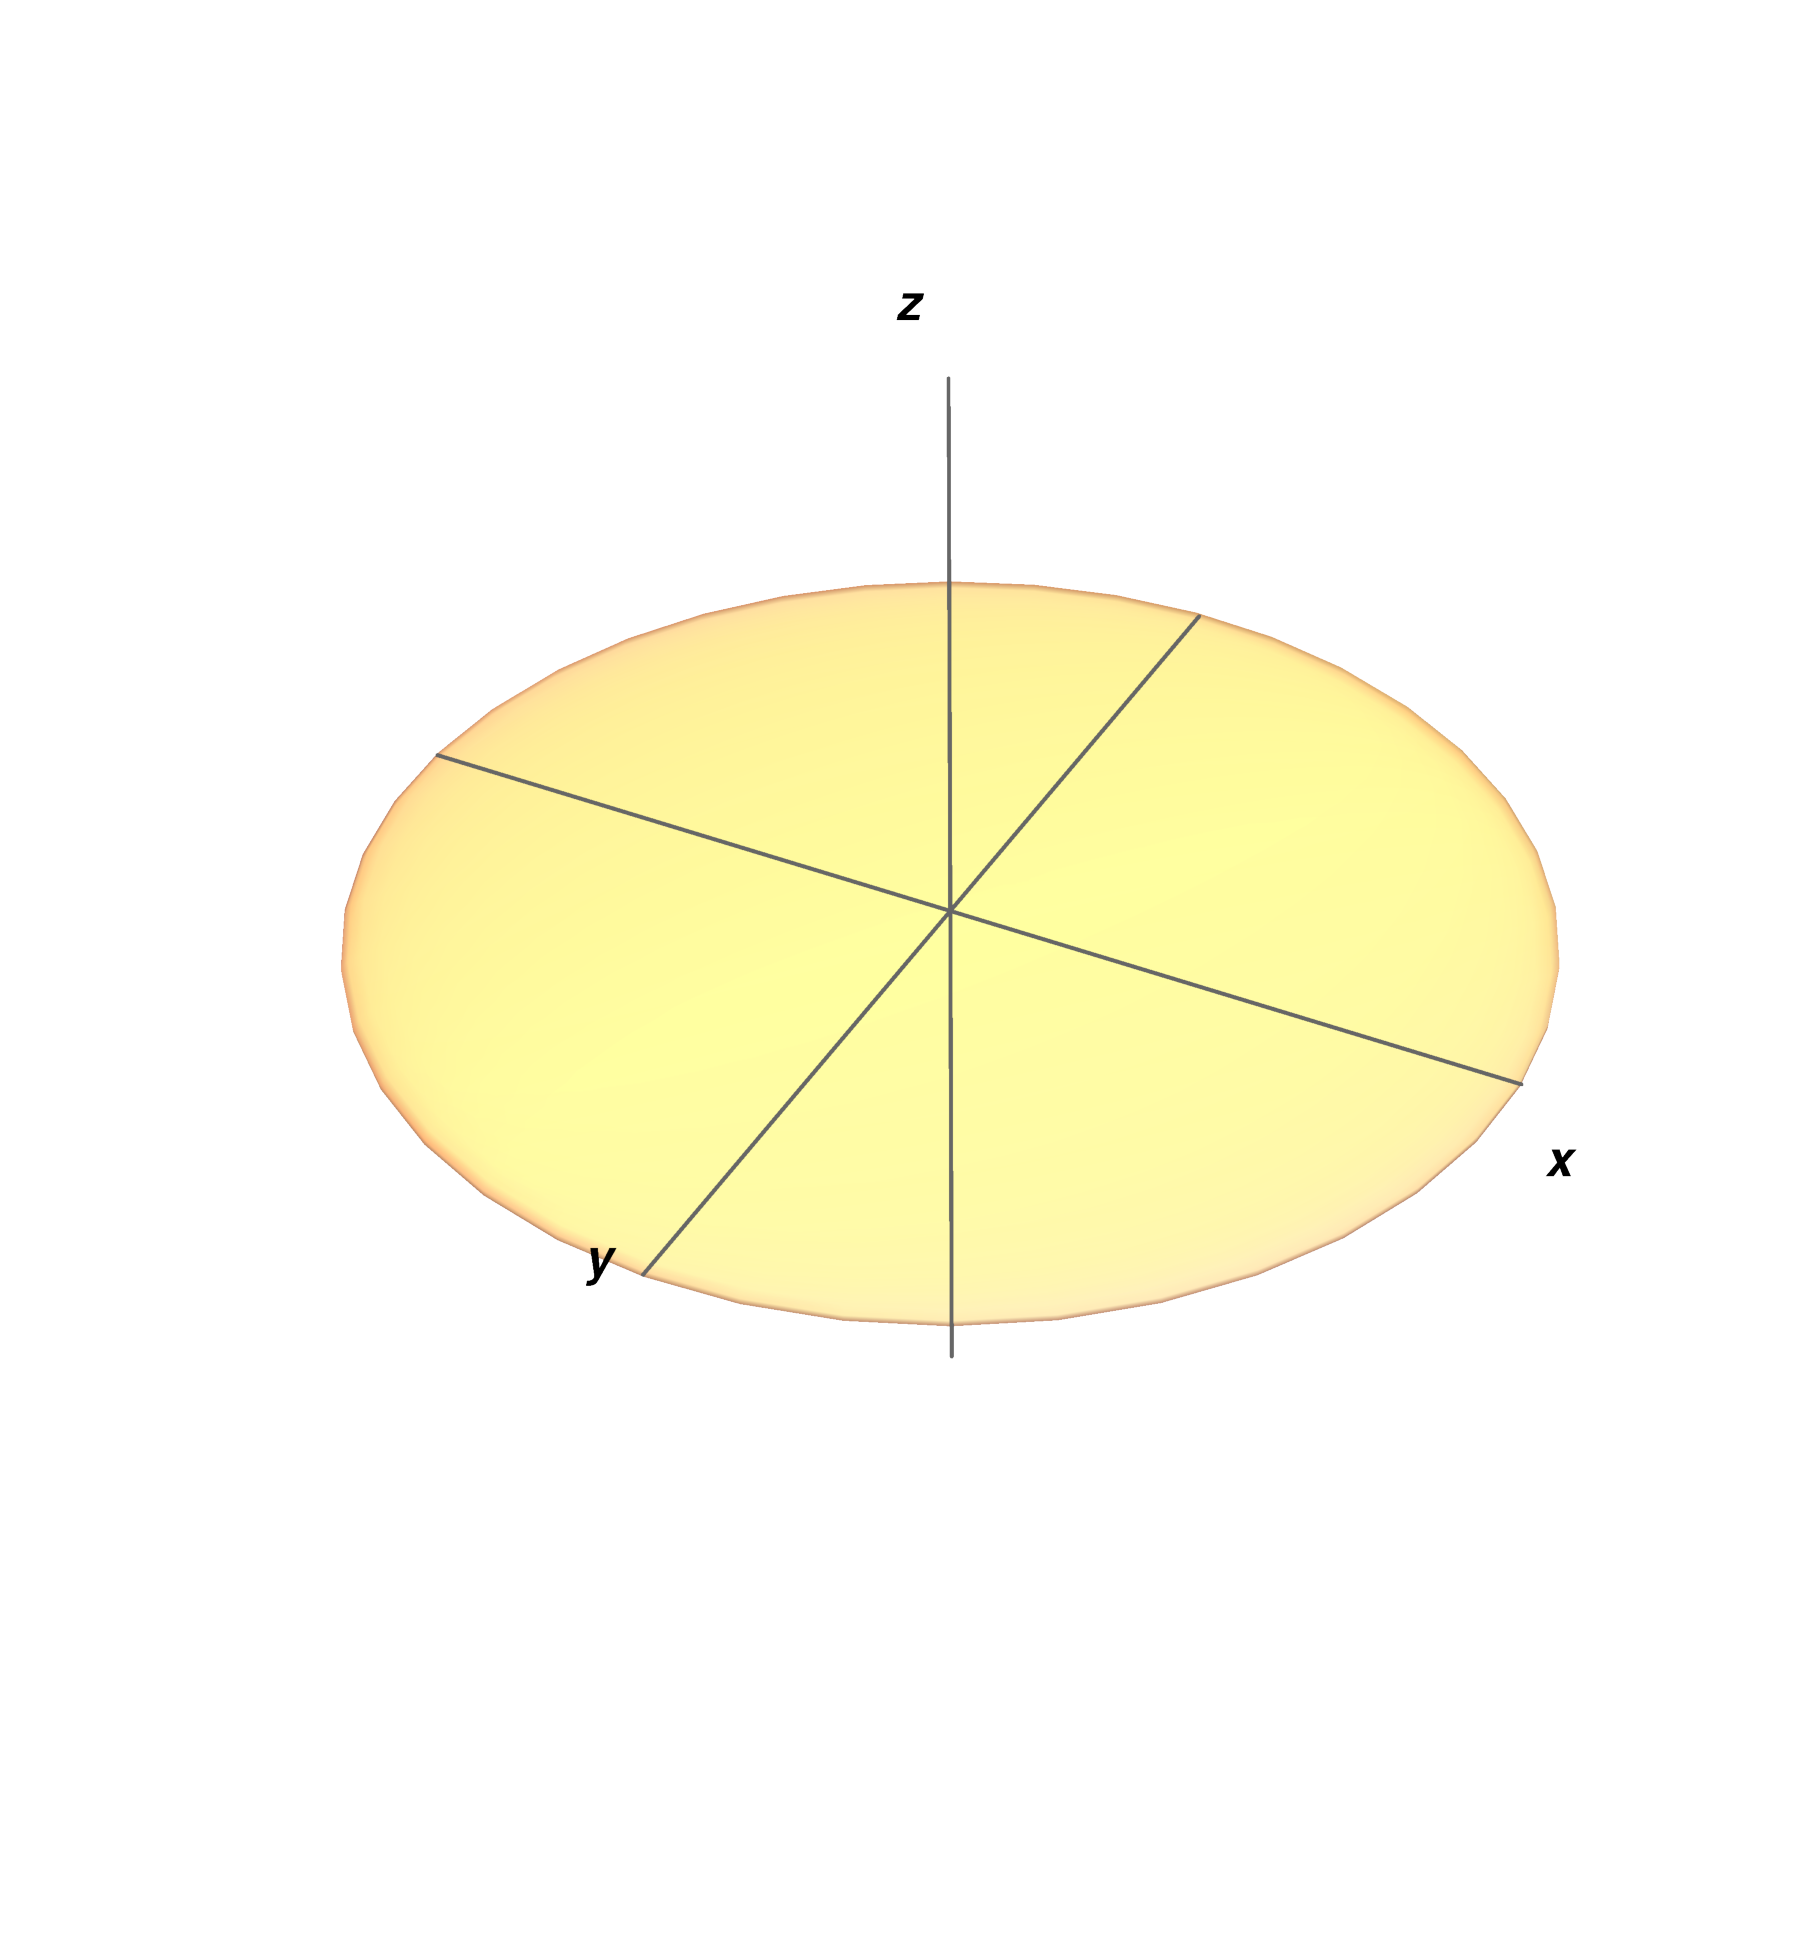
\includegraphics[width=6cm]{DiskXY}
\end{minipage}
\caption{
Deformación de la esfera de Bloch a un disco sobre el plano $XY$.}
\label{fig:qtm-op-motivation}
\end{figure} % }}}

El estado máximamente entrelazado de 2 qubits es
$\ket{\phi}=\qty(\ket{0}+\ket{1})/\sqrt{2}$~\cite{bengtsson_zyczkowski_2017}.
Ya que conocemos cómo transforma $\E_z$ a las componentes de 
la matriz de densidad escrita en la base de Pauli es necesario calcular 
la representación de $\dyad{\phi}{\phi}$ en esa base.
Las componentes $r_{ij}$ se calculan a partir de las
proyecciones de $\dyad{\phi}{\phi}$ sobre los elementos 
$\sigma_i\otimes\sigma_j$ usando el producto interno
de Hilbert-Schmidt $\Tr\qty(\pauli{i}{j}\dyad{\phi}{\phi})$.
Así, se encuentra que
\begin{align}
\dyad{\phi}{\phi}=
\pauli{0}{0}+\pauli{1}{1}-\pauli{2}{2}+\pauli{3}{3}.
\end{align}

Ya que $\E_z$ borra la componente $z$ del vector de Bloch, 
entonces la acción de $\E_z\otimes\1$ debe ser tal que borra 
las componentes de la forma $r_{3j}$ de $\dyad{\phi}{\phi}$, 
por lo cual
\begin{align}
\E_z\otimes\1 \qty({\rho}^{\phi})=
\pauli{0}{0}+\pauli{1}{1}-\pauli{2}{2};
\end{align}
y, transformando de vuelta a la base computacional,
\begin{align}
\E_z\otimes\1 \qty(\dyad{\phi}{\phi})=
\mqty( 
\frac{1}{4} & 0 & 0 & \frac{1}{2} \\
0 & \frac{1}{4} & 0 & 0 \\
0 & 0 & \frac{1}{4} & 0 \\
\frac{1}{2} & 0 & 0 & \frac{1}{4} \\
).
\end{align}
La matriz  $\E_z\otimes\1\qty(\dyad{\phi}{\phi})$ tiene un 
eigenvalor igual a $-1/4$ y, por lo tanto, no es una matriz de densidad.  
Dicho de otro modo, $\E_z\otimes\1\qty(\dyad{\phi}{\phi})$ 
no cumple con una de las condiciones para representar un estado físico
de un sistema de 2 qubits. Hemos mostrado con este ejemplo que la completa 
positividad es una condición más fuerte a la de la positividad para 
asegurar que todos los estados de un sistema, incluyendo a 
cualquier posible estado entrelazado con otro sistema, se transforman
en estados físicos.

Ahora vamos a establecer la condición de completa positividad 
de forma precisa. Se dice que una operación $\E$ es CP si 
y sólo si, para cualquier extensión arbitraria de dimensión $K$ 
del espacio de Hilbert $(\hi_N \rightarrow \hi_N \otimes \hi_K)$ 
el operador $\E\otimes\1_K$ es positivo~\cite{bengtsson_zyczkowski_2017}. 
Con esta condición las restricciones sobre un canal cuántico 
para que este describa una evolución física están completas.

Un canal cuántico es un mapeo lineal que  (1) preserva las características
de las matrices de densidad y (2) es completamente positivo. 
En la literatura se suele utilizar el término operaciones 
completamente positivas que preservan la traza 
(CPTP) para referirse a los canales 
cuánticos~\cite{bengtsson_zyczkowski_2017}. 
Ahora que hemos establecido las condiciones que satisfacen los
canales cuánticos vamos a presentar en la siguiente sección 
dos formas distintas, pero equivalentes, de representar a un canal 
cuántico: como superoperador y la forma de Kraus.


% }}}
\section{Representaciones de los canales cuánticos} % {{{
\label{sec:qtm-channels-representation}
\esqueleto{Enunciar que existen las representaciones de 
Kraus y de superoperador. Copy-paste de las secciones en las 
que hablamos de las representaciones en el informe final. Planeo
dejar sólo un ejemplo y matar los ejemplos de las dos representaciones
en un tiro.}

Los canales cuánticos pueden representarse como superoperadores
o en la representación de suma de operadores de Kraus. 
La matriz de densidad es un operador que actúa sobre el espacio 
de Hilbert, por consiguiente, la ecuación \eqref{eq:E(rho)} 
sugiere que $\E$ es un operador que actúa sobre el espacio 
de Hilbert-Schmidt (espacio en el que viven las matrices de densidad). 
A esta clase de operadores es a los que se les conoce como 
superoperadores~\cite{preskill1998lecture}.
Por otro lado, la representación de Kraus es una forma de 
representar a un canal cuántico con operadores que pertenecen
al mismo espacio en el que se contienen las matrices de densidad.

Un superoperador actúa sobre la matriz de densidad 
como un vector columna. Por ello, discutiremos un procedimiento 
para `vectorizar' a la matriz de densidad.
Consideremos una matriz de densidad $\hat{\rho}$ de dimensión $d\times d$.
La matriz $\hat{\rho}$ puede escribirse como 
un vector columna $\vec{\rho}$, con $d^2$ elementos, 
ordenando los elementos de matriz según la ecuación  
\begin{align}
\rho_k=\hat{\rho}_{ij}, 
\label{eq:matrix-to-vector}
\end{align}
donde $k=\qty(i-1)d+j$, con $i,j=,1,\ldots,d$. 

Para establecer más adelante una manera de evaluar la CP de una operación 
lineal vamos a introducir a continuación una notación de 4 índices para 
etiquetar a los elementos de matriz de un operador que actúa 
sobre un espacio bipartito y una transformación conocida como 
\textit{reshuffle} para reordenar a una matriz. 
Supongamos que $U$ es un operador 
que actúa sobre un espacio de Hilbert 
$\hi$ de la forma $\hi=\hi_M\otimes\hi_N$.
Consideremos una base ortonormal $\ket{m}$ de $\hi_M$ 
y una base ortonormal $\ket{\mu}$ de $\hi_N$. 
Los productos $\ket{m}\otimes\ket{\mu}$ definen a una base
ortonormal del espacio compuesto $\hi$. 
Nótese el uso de letras latinas para los índices del
primer subsistema y letras griegas para los índices del segundo. 
Un elemento de matriz de $U$ se puede etiquetar como
\begin{align}
U_\ind{m\mu}{n\nu}=\matrixel{m\otimes \mu}{U}{n\otimes \nu}.
\label{eq:4indices}
\end{align}
En esta notación de cuatro índices la transformación de \textit{reshuffle}, 
para reordenar a una matriz  $U$, se define 
como~\cite{bengtsson_zyczkowski_2017}
\begin{align}
U^R_\ind{m\mu}{n\nu} = U_\ind{mn}{\mu\nu}.
\label{eq:R-4ind}
\end{align}
Con esta nueva notación y una definición de 
la transformación de \textit{reshuffle}
contamos con las herramientas necesarias para establecer 
las condiciones que un superoperador $\E$ debe satisfacer 
para ser un canal cuántico.

Un canal cuántico es una operación lineal completamente
positiva que preserva las características de la matriz de densidad.
Es decir, un canal cuántico transforma a la matriz de densidad de
tal manera que preserva su (1) Hermiticidad, (2) traza unitaria y 
(3) positividad semidefinida. Para que esto se satisfaga, un 
canal cuántico $\E$ debe cumplir~\cite{bengtsson_zyczkowski_2017}:
\begin{align}
\txt{(i)}&& \rho'=\qty(\rho')^{\dagger}&&\Leftrightarrow
    && \E_\ind{m\mu}{n\nu}=\E_\ind{\mu m}{\nu n}^*,&&
    \label{eq:H-condition}\\
\txt{(ii)}&&\Tr(\rho')=1
    &&\Leftrightarrow&&  \sum_{m}\E_\ind{mm}{n\nu}=\delta_{n\nu},\\     
\txt{(iii)}&&\rho'\geq0
    &&\Leftrightarrow&&  \sum_{n\nu}\E_{\ind{m\mu}{n\nu}}\rho_{n\nu}\geq0 &
    \text{\hspace{8pt}cuando\hspace{4pt}} \rho>0.
    \label{eq:positivity-condition}
\end{align}
Adicionalmente, para evaluar la completa positividad de $\E$ es 
necesario introducir a la matriz de Choi $D_{\E}$ de un canal cuántico.
La matriz $D_{\E}$ se define como la matriz resultante de 
aplicar la transformación de \textit{reshuffle} al superoperador $\E$,
es decir, $D_{\E}=\E^{R}$~\cite{bengtsson_zyczkowski_2017}.
Finalmente, la condición de CP de $\E$, utilizando a su matriz de Choi, 
está establecida en el siguiente teorema.
\begin{thm}{Teorema de Choi.}\label{thm:choi-CP}
Un superoperador lineal $\E$ es completamente positivo si y sólo si 
su matriz de Choi asociada $D_{\E}$ es positiva semidefinida.
\end{thm}
\begin{proof}
Vamos a presentar la demostración expuesta por Bengtsson
en~\cite[p. 281]{bengtsson_zyczkowski_2017}.
La matriz de Choi $D_{\E}$ de un 
canal cuántico $\E$ es una matriz Hermítica que 
actúa sobre el espacio de Hilbert-Schmidt $\mathcal{H}_{N^2}$
(espacio de las matrices de dimensión $N^2\times N^2$). 
Utilizando el teorema de descomposición 
espectral~\cite{nielsen_chuang_2011},
\begin{align}
D_{\E}&=\sum_{i}\lambda_i\dyad{\chi_i}{\chi_i}
&
D_{\ind{mn}{\mu\nu}}&=\sum_i\lambda_i
\chi^i_{mn}\qty(\chi_{\mu\nu}^i)^*,
\end{align}
donde los eigenvalores $\lambda_i\in\mathbb{R}$. Ahora consideremos
la acción de $\E\ot \1_N$ sobre un estado puro $z_{nn'}z^*_{\nu\nu'}$,
\begin{align}
\rho'_{mm'\mu\mu'}&=
\sum_{n,n',\nu,\nu'}
\E_{\ind{m\mu}{n\nu}}\delta_{\ind{m'\mu'}{n'	\nu'}}z_{nn'}z^*_{\nu\nu'}
=
\sum_{n,\nu}
\E_{\ind{m\mu}{n\nu}}z_{nm'}z^*_{\nu\mu'},
\end{align}
donde $\delta_{\ind{m'\mu'}{n'	\nu'}}=\delta_{m'n'}\delta_{\mu'\nu'}$,
\begin{align}
\sum_{n,\nu}\E_{\ind{m\mu}{n\nu}}z_{nm'}z^*_{\nu\mu'}&=
\sum_{n,\nu}D_{\ind{mn}{\mu\nu}}z_{nm'}z^*_{\nu\mu'}\nonumber\\
\rho'_{mm'\mu\mu'}&=
\sum_{n,\nu,i}\lambda_{i}
\chi^i_{mn}z_{nm'}\qty(\chi_{\mu\nu}^iz_{\nu\mu'})^*,
\end{align}
donde utilizamos $\E_{\ind{m\mu}{n\nu}}
=\E^R_{\ind{mn}{\mu\nu}}
=D_{\ind{mn}{\mu\nu}}$.
Finalmente, para evaluar que $\rho'$ sea una matriz de densidad positiva 
calculamos sus elementos de matriz con un vector arbitrario~$y_{mm'}$
para encontrar la condición que se debe de satisfacer,
\begin{align}
\sum_{m,m',\mu,\mu'}
y_{mm'}\rho'_{mm'\mu\mu'}y_{\mu\mu'}=
\sum_{m,m',n,n'}\lambda_i\abs{
y_{mn'}\chi^i_{mn}z_{nm'}}^2
\geq0,
\end{align}
entonces $\lambda_i\geq1$. Por consiguiente, la matriz 
de Choi $D_{\E}$ debe ser positiva semidefinida para que $\rho'$ 
también lo sea.
\end{proof}
En resumen, las condiciones \eqref{eq:H-condition} 
a \eqref{eq:positivity-condition}, más el teorema \eqref{thm:choi-CP},
establecen las restricciones sobre el superoperador $\E$ para que sea
un canal cuántico~\cite{bengtsson_zyczkowski_2017}.

Por el otro lado, un canal cuántico $\E$ también puede escribirse
en la representación de suma de operadores.
En 1971, Karl Kraus introdujo esta representación como resultado
del teorema de Stinespring \cite{bengtsson_zyczkowski_2017}.
La representación de Kraus de un canal cuántico reescribe
a la ecuación \eqref{eq:E(rho)} como
$\E\qty(\rho)=\sum_k E_k\rho E_k^{\dagger}$,
para algún conjunto de operadores $\{E_k\}$ 
que satisfacen la condición 
$\sum _kE_k^{\dagger}E_k\leq\1$~\cite{nielsen_chuang_2011}. 
Esta representación se relaciona con el superoperador $\E$ por
medio de la matriz de Choi.

La representación de Kraus no es única y, por ello, es de interés
determinar un conjunto $\{E_k\}$ de operadores canónicos de $\E$.
Se puede encontrar un conjunto de operadores canónicos de Kraus de 
un canal cuántico $\E$ a partir de los eigenvectores normalizados 
$\ket{\chi_k}$ de la matriz de Choi reordenados como matrices 
mediante el proceso inverso
establecido en \eqref{eq:matrix-to-vector}~\cite{bengtsson_zyczkowski_2017}.
Además, la raíz cuadrada de los eigenvalores $\sqrt{\lambda_k}$ de 
$D_{\E}$ proporcionan los pesos de los operadores canónicos $E_k$.

\textbf{Forma canónica de Kraus.} Un mapeo completamente 
positivo $\E:\mathcal{M}^{(N)}\to\mathcal{M}^{(N)}$ se
puede escribir como
\begin{align}
\rho \longrightarrow \rho' = 
\sum_{k=1}^{r\leq d^2}\lambda_k\chi_k\rho\chi_k^{\dagger}
= \sum_{i=1}^rE_k\rho E_k^{\dagger},
\label{eq:Kraus-canonical}
\end{align}
donde $r$ es el rango de $D_{\E}$ y $\chi_k$ sus eigenvectores
$\ket{\chi_k}$ reordenados como matrices. Esto quiere decir que 
$E_k=\sqrt{\lambda_k}\chi_k$. Además, los 
operadores $E_k$ deben satisfacer la condición
\begin{align}
  \Tr\qty(E_i^{\dagger}E_j)=d_i\delta_{ij}.
  \label{eq:Tr-Kraus-canonical}
\end{align}
Si canal cuántico $\E$ preserva la $\Tr \rho$, se cumple que
\begin{align}
  \sum_kE_k^{\dagger}E_k=\1
  \hspace{0.5cm}\Rightarrow\hspace{0.5cm}
  \sum_{k=1}^r\lambda_k=N .
  \label{eq:completeness-Kraus-canonical}
\end{align}
Se conoce como rango de Kraus al número de operadores 
en la forma canónica. Es decir, el número de términos en la sumatoria
en \eqref{eq:Kraus-canonical}. Por consiguiente, el rango de 
Kraus de $\E$ es igual al rango de su matriz de Choi 
$D_{\E}$~\cite{bengtsson_zyczkowski_2017}.

Con esto completamos los fundamentos teóricos para estudiar 
el problema de las operaciones PCE a partir del siguiente capítulo. 
Primero presentamos a la matriz de densidad como una herramienta 
para representar a los estados cuánticos. Luego, expusimos la teoría 
de los canales cuánticos para estudiar la dinámica de los sistemas 
cuánticos abiertos. Un canal cuántico es una operación
completamente positiva que preserva las características de la 
matriz de densidad. Ahora nos vamos a centrar en estudiar una 
dinámica muy particular de los sistemas de qubits.
% }}}
%%% Lo que está comentado abajo era parte del modelo, puede ser útil  después  {{{
%%%%%%%%%%%%%%%%%%%%%%%%%%%%%%%%%%%%%%

%En adición a los conjuntos de puntos que se trabajan con normalidad
%en Matemáticas ~---puras y aplicadas---, se tendrá que hacer uso
%frecuentemente de los conjuntos de conjuntos, si por ejemplo $X$ es
%la recta real, como un intervalo es un conjunto de puntos, es decir
%un subconjuto de $X$, se tendrá que el conjunto de todos los
%intervalos es un conjunto de conjuntos.
%
%En especial, cuando una clase hace referencia a subconjuntos del
%conjunto $X$, la llamaremos \textbf{familia}. En especial el
%\textbf{conjunto potencia} $\mathcal{P} (X)=\{A\mid A\subseteq X\}$
%es una familia de $X$. Asimismo, se definirá el \textbf{complemento}
%de $A$ por \[A^c=\{x\mid x\notin A\}.\]
%
%\begin{defn}\label{dfcp28} Una \textbf{función de selección}
%para un conjunto $X$ es una función $f$ la cual asocia a cada
%subconjunto no vacío $E$ de $X$ un elemento de $E$: $f(E)\in E$.
%\end{defn}
%
%\begin{axm}[de selección]\label{choice} Para cualquier conjunto
%existe una función de selección.
%\end{axm}
%
%\begin{rem} Con frecuencia el axioma~\ref{choice} se presenta en
%la forma: para cada $E\in \mathcal{P}(X)\setminus\{\nada\}$,
%elegimos un elemento $x\in E$. Asimismo, es equivalente al lema de
%Zorn, para más detalles consultar
%~\cite[p. 97]{Halmo},~\cite[p. 338]{Haus} o~\cite[p. 14]{Hewit}.
%\end{rem}
%
%Una \textbf{clase disjunta} es una clase {\boldmath $A$} de
%conjuntos tal que para cualquier par de conjuntos distintos de
%{\boldmath $A$} son disjuntos, en este caso nos referiremos a la
%unión de conjuntos de {\boldmath $A$} como \textbf{unión disjunta}.
%
%Si $E$ es un subconjunto de $X$, la función $\chi _E$ definida para
%$x\in X$ por la relación:
%\begin{equation}\label{eq0}
%    \chi_E(x)= \begin{cases}
%    1, & \mbox{si } x\in E, \\
%    0, & \mbox{si } x\notin E.
%    \end{cases}
%\end{equation}Es llamada \textbf{función característica}
%del conjunto $E$. La correspondencia entre los conjuntos y sus
%funciones características es inyectiva, y todas las propiedades de
%conjuntos y operaciones entre conjuntos pueden ser expresadas por
%medio de funciones características. 
%
%%%%	TABLA CORTA, ÚNICAMENTE LLEVA LÍNEAS HORIZONTALES PARA SEPARAR BLOQUES
%
%\begin{table}[ht]
%\caption[título optativo de la tabla]{Propiedades de los espacios $L^p$. Fuente: tomada de \cite[Cap. 3]{Brez}.}\label{tablaLp}
%\centering
%\begin{tabular}{cccc}
%\hline
%Espacio & Reflexivo\footnote{En el sentido topológico.} & Separable & Dual \\ \hline %\hline
%$L^p$, $1<p<\infty$  & Si & Si & $L^q$, $1/p+1/q=1$ \\
%$L^1$ & No & Si & $L^\infty$ \\
%$L^\infty$ & No & No & $L^1 \varsubsetneq (L^\infty)’$ \\ \hline
%\end{tabular}
%\end{table}\footnotetext{En el sentido topológico.} 
%
%\begin{defn}\label{dfcp1}Si $\su En$ es una sucesión de
%conjuntos, definiremos los conjuntos $\overline{\lim } E_n$ y
%$\underline{\lim } E_n$ de la siguiente forma:
%\[\begin{array}{cc}
%  \overline{\lim} E_n=\limsup \limits_{n\rightarrow \infty}E_n =
%  \bigcap \limits_{n=1}^\infty \Union Ein \infty ,&
%  \underline{\lim} E_n=\liminf \limits_{n\rightarrow \infty}E_n =
%  \bigcup \limits_{n=1}^\infty \Inter Ein \infty \\
%\end{array}\] y los llamaremos \textbf{límite superior} y
%\textbf{límite inferior}, respectivamente, de la sucesión $\su En$.
%Si tenemos $\overline{\lim} E_n = \underline{\lim} E_n$, usaremos la
%notación $\lim_n E_n$ para este conjunto. Si la sucesión es tal que
%$E_n\subset E_{n+1},\ n=1,2,\dots$ le llamaremos \textbf{creciente}
%y se denotará por $E_n\!\!\uparrow$ y su límite será $\lim
%\limits_{n\rightarrow \infty}E_n = \union En1 \infty$; si es tal que
%$E_n\supset E_{n+1},\ n=1,2,\dots$ le llamaremos
%\textbf{decreciente} y se denotará por $E_n\!\!\downarrow$ y su
%límite será $\lim \limits_ {n\rightarrow \infty}E_n = \inter En1
%\infty$. En ambos casos nos referiremos a ella como
%\textbf{monótona}.\end{defn}
%
%
%\begin{defn}\label{dfcp2}Sea $f$ una aplicación definida del conjunto
%$X$ al conjunto $Y$, es decir $f:X\To Y$. Para cualquier subconjunto
%$T\subseteq Y$, definimos la \textbf{imagen inversa} de $T$, bajo
%$f$, denotada por $\ff (T)$, como sigue:
%\[\ff (T)=\{s\in X\mid f(s)\in T\}.\]\end{defn} 
%
%\begin{thm}\label{thcp1}Para la aplicación $\ff :{\cal{P}} (Y)
%\To {\cal{P}} (X)$ se tienen las propiedades siguientes:
%\begin{enumerate}
%    \vspace{0pt} \item $\ff(\bigcup_j T_j) = \bigcup_j
%    \ff(T_j)$.
%    \vspace{0pt} \item $\ff(\bigcap_j T_j) = \bigcap_j
%    \ff(T_j)$.
%    \vspace{-6pt} \item Si $T_1\cap T_2=\nada$, entonces
%    $\ff(T_1)\cap \ff(T_2) = \nada$.
%    \vspace{-6pt} \item $\ff(T^c) = [\ff(T)]^c$.
%    \vspace{-6pt} \item $\ff(\nada) = \nada$.
%    \vspace{-6pt} \item $\ff(Y) = X$.
%\end{enumerate}
%\end{thm}
%
%
%Las propiedades (1) y (3) del teorema~\ref{thcp1} establecen las
%condiciones para la unión disjunta en una familia en $Y$. Sea ahora
%$\Df$ una familia cualquiera de subconjuntos de $Y$, y definamos la
%familia $\ff (\Df)$ de subconjuntos de $X$ como
%sigue:\begin{equation}\label{eq1}
%    \ff(\Df) = \{A\subseteq X \mid
%A = \ff(T) \mbox{ para algún } T\in \Df\} = \{\ff(T) \mid T\in
%\Df\}.
%\end{equation}
%
%El sistema de numeros reales extendido o \textbf{recta real
%extendida} es el conjunto definido por $\RR\df\R \cup \{-\infty,
%+\infty\}$, con la siguiente relación de orden: para $a\in \R$
%tenemos $-\infty <a< +\infty$. La topología para este conjunto se
%define por declarar como abiertos a los siguientes conjuntos:
%$(a,b),\ [-\infty,b),\ (a,+\infty]$ y cualquier unión de conjuntos
%de este tipo. Cuando se haga referencia a los \textbf{numeros reales
%extendidos} o \textbf{valor real extendido}, se estará hablando de
%los numeros reales y de los símbolos $\pm\infty$. Cuando trabajamos
%con teoría de la integración, nos encontraremos con $\infty$, una
%razón es que algunas veces trataremos de integrar sobre conjuntos de
%medida infinita, este es caso de la recta real.
%
%Por tal motivo, se hacen las siguientes definiciones para
%facilitar su manejo: $a+\infty = \infty+a \df \infty$ si $0\leq a
%\leq \infty$,~y
%\begin{equation}\label{eq4}
%    a\cdot \infty = \infty \cdot a
%\df\begin{cases}
%  \infty, & \mbox{si } 0 < a \leq \infty \\
%  0, & \mbox{si } a = 0 \\
%\end{cases}
%\end{equation}las leyes de cancelación se tratan
%así: $a+b = a+c\ \Rightarrow\ b=c\ $ y $a\cdot b =a\cdot c\
%\Rightarrow\ b=c$ sólo cuando $0 < a < \infty$. 
%
%\begin{defn}\label{dfcp3}Sea $\su aj$ una sucesión en la recta
%real extendida, y sean $b_k = \sup\{a_k,a_{k+1},a_{k+2}\dots\},\
%k=1,2,3,\dots$, y $\beta = \inf\{b_1,b_2,b_3,\dots\}$. Entonces
%llamaremos a $\beta$ el \textbf{límite superior} de $\su aj$, y
%escribiremos $\beta = \limsup \limits_{j\rightarrow \infty}(a_j)$.
%El \textbf{límite inferior} se define análogamente, al intercambiar
%$\sup$ e $\inf$ en las anteriores definiciones; notemos que \[\liminf
%\limits_{j\rightarrow \infty}(a_j) = -\limsup \limits_{j\rightarrow
%\infty}(-a_j).\] Si $\su aj$ converge, entonces tenemos $\liminf
%\limits_{j\rightarrow \infty}(a_j) = \limsup \limits_{j\rightarrow
%\infty}(a_j) = \lim \limits_{j\rightarrow
%\infty}(a_j)$.\end{defn}
%
%\begin{prp}\label{prcp1}Si $0\leq a_1\leq a_2\leq \cdots$,
%$0\leq b_1\leq b_2\leq \cdots$, tales que $a_j \To a$ y $b_j \To
%b$. Entonces $a_j b_j \To ab$.
%\end{prp}
%
%\begin{defn}\label{dfcp4}Supongamos que $\su fj$ es una sucesión de
%funciones de valor real extendido en un conjunto $X$. Entonces
%$\sup_j f_j$ y $\limsup \limits_{j\rightarrow \infty} f_j$ son las
%funciones definidas en $X$ por:
%\[\left(\sup_j f_j\right)(x)\df \sup_j(f_j(x)),\quad \left(\limsup
%\limits_{j \rightarrow \infty} f_j\right)(x)\df \limsup \limits_{j
%\rightarrow \infty}(f_j(x)).\] Si $f(x)=\lim \limits_{j \rightarrow
%\infty} f_j(x)$, y asumimos que el límite existe para cualquier
%$x\in X$, entonces llamaremos a $f$ el \textbf{límite puntual} de la
%sucesión $\su fj$ y hablaremos de \textbf{convergencia puntual} en
%este contexto.\end{defn}
%
%\begin{figure}[ht]
%\centering
%\label{fig:analisisGraficoModelo3}
%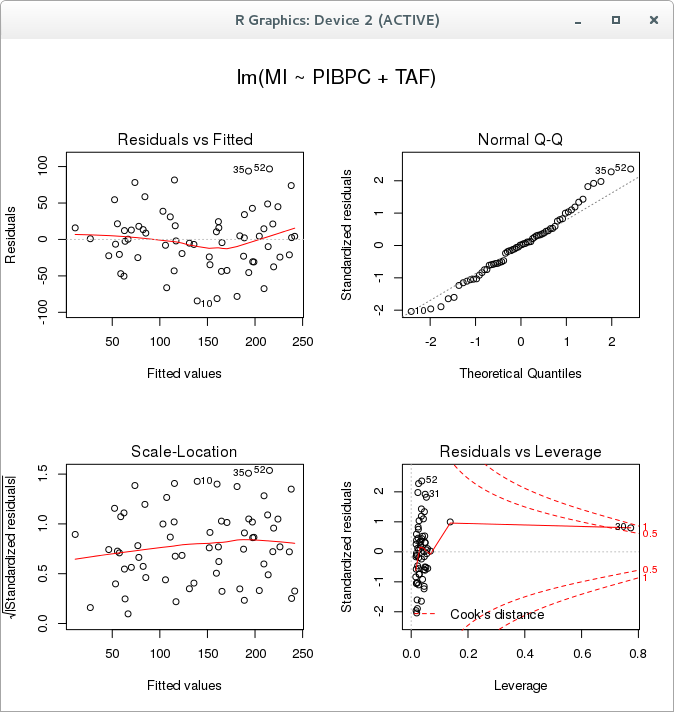
\includegraphics[width=0.9\linewidth]{analisisGraficoModelo3}\\
%\caption[Titulo en el índice de figuras (opcional)]{Título en el 
%documento. Las imágenes pueden ser raster (de preferencia jpg, png 
%con buena resolución para imprimir) o vectorial (convertir a pdf, en 
%este caso la resolución no afecta) Fuente: imagen tomada de~\cite{liu}.}
%\end{figure}
%
%
%\begin{lem}\label{lmcp11}Sean $z,w \in \C$, $1 < p \leq 2$ y $1/p +
%1/q = 1$. Entonces tenemos \[\abs{z+w}^q + \abs{z-w}^q \leq 2 (|z|^p
%+ |w|^p)^{\frac{1}{p-1}}.\]
%\end{lem}
%
%\begin{proof} Consultar~\cite[p. 227]{Hewit}. \end{proof}
%
%\begin{defn}\label{dfcp5}Sea $f:X\To \RR$ una aplicación. Se definen
%las aplicaciones $f^+\!\df\max\{f,0\}$, $f^-\!\df-\min\{f,0\}$, a
%$f^+$ y $f^-$ se les llama la \textbf{parte positiva y negativa} de
%$f$, respectivamente.
%\end{defn}
%
%
%\begin{prp}\label{prcp2}Para cualquier aplicación $f:X\To \R$
%denotaremos su valor absoluto con $\abs f$, entonces tenemos
%\[\abs f=f^++f^-,\quad f=f^+-f^-.\]
%\end{prp}
%
%% --------------->  
%
%\section{Tablas y Gráficas}
%
%Las tablas y gráficas deben tener un título \verb|\caption{text}| que la identifique, debe especificar la \textbf{fuente}, y una etiqueta \verb|\label{text}| para hacer referencias cruzadas dentro del documento.
%
%%% TABLAS LARGAS LLEVAN TODAS LAS DIVISIONES DE LOS BLOQUES
%\subsection{Tablas}
%
%\begin{longtable}{|l|l|l|l|l|}
%\caption[]{Diccionario de datos, tabla \textit{marn} (continuación)} \\ \hline
%
%\multicolumn{1}{|c|}{\textbf{Name}} & \multicolumn{1}{c|}{\textbf{Data type}} & \multicolumn{1}{c|}{\textbf{Not Null?}} & \multicolumn{1}{c|}{\textbf{Primary key?}} & \multicolumn{1}{c|}{\textbf{Default}} \\ \hline \endhead
%	\caption[Diccionario de datos, tabla \textit{marn}]{Diccionario de datos, tabla \textit{marn}. Fuente: obtenida de pgAdminIII}\label{data:marn} \\ \hline
%
%	\multicolumn{1}{|c|}{\textbf{Name}} & \multicolumn{1}{c|}{\textbf{Data type}} & \multicolumn{1}{c|}{\textbf{Not Null?}} & \multicolumn{1}{c|}{\textbf{Primary key?}} & \multicolumn{1}{c|}{\textbf{Default}} \\ \hline \endfirsthead 
%
%	id & \textit{integer} & \textit{Yes} & \textit{Yes} & \textit{nextval('marn\_id\_seq'} \\ %\hline
%
%	 &  &  &  & \textit{::regclass)}\footnote{Note que la tabla es mas ancha que lo preestablecido. Procure diseñar elementos acordes con el espacio preestablecido.} \\ \hline
%
%	\multicolumn{ 5}{|l|}{Clave primaria que  obtendrá su valor de forma secuencial al ingresar un nuevo registro} \\ \hline
%		lista\_tax & \textit{text} & \textit{No} & \textit{No} & \textit{} \\ \hline
%
%	\multicolumn{ 5}{|l|}{Clasificación del proyecto en base al Listado Taxativo del MARN} \\ \hline
%		no\_marn & \textit{text} & \textit{No} & \textit{No} & \textit{} \\ \hline
%
%	\multicolumn{ 5}{|l|}{Numero de expediente asignado por el MARN} \\ \hline
%		date0 & \textit{date} & \textit{No} & \textit{No} & \textit{} \\ \hline
%
%	\multicolumn{ 5}{|l|}{Día del ingreso del expediente del proyecto (instrumento ambiental) en el MARN} \\ \hline
%		notas & \textit{text} & \textit{No} & \textit{No} & \textit{} \\ \hline
%
%	\multicolumn{ 5}{|l|}{Observaciones} \\ \hline
%		no\_res\_ap & \textit{text} & \textit{No} & \textit{No} & \textit{} \\ \hline
%
%	\multicolumn{ 5}{|l|}{Numero de resolución aprobatoria del proyecto por el MARN%
%	\footnote{Note que en esta línea la tabla se corta y continua en la siguiente página. 
%	Utilizar paquete \textsf{longtable} y ambiente \textit{longtable}.}} \\ \hline
%		date\_res\_ap & \textit{date} & \textit{No} & \textit{No} & \textit{} \\ \hline
%
%	\multicolumn{ 5}{|l|}{Día de emisión de la resolución aprobatoria por el MARN} \\ \hline
%		date0\_fianza & \textit{date} & \textit{No} & \textit{No} & \textit{} \\ \hline
%
%	\multicolumn{ 5}{|l|}{Día de emisión de fianza del proyecto.} \\ \hline
%		no\_res\_fianza & \textit{text} & \textit{No} & \textit{No} & \textit{} \\ \hline
%
%	\multicolumn{ 5}{|l|}{Numero de la resolución de aceptación de fianza por el MARN} \\ \hline
%		date1\_fianza & \textit{date} & \textit{No} & \textit{No} & \textit{} \\ \hline
%
%	\multicolumn{ 5}{|l|}{Fecha de inicio de fianza} \\ \hline
%		date2\_fianza & \textit{date} & \textit{No} & \textit{No} & \textit{} \\ \hline
%
%	\multicolumn{ 5}{|l|}{Fecha de finalización de fianza (renovación)} \\ \hline
%		lic\_ambiental & \textit{text} & \textit{No} & \textit{No} & \textit{} \\ \hline
%
%	\multicolumn{ 5}{|l|}{Numero de licencia ambiental} \\ \hline
%		date\_lic\_ambiental & \textit{date} & \textit{No} & \textit{No} & \textit{} \\ \hline
%
%	\multicolumn{ 5}{|l|}{Fecha de finalización de ultima licencia ambiental} \\ \hline
%		proyecto\_id & \textit{integer} & \textit{Yes} & \textit{No} & \textit{} \\ \hline
%
%	\multicolumn{ 5}{|l|}{Enlace con la tabla proyecto\_id} \\ \hline
%\end{longtable}

% }}}


